% Chapter 5

\chapter{Experiments} % Methodology

\label{Chapter5} % For referencing the chapter elsewhere, use \ref{Chapter5} 

In this chapter we present the results of the experiments conducted and discus the refinements made to the models as a result of the experiments. We start with a summary of the best results obtained by each method before going into a more in-depth evaluation in the subsequent sections.

\section{Results summary}

Looking at the F1-score we see that the RNN model performed the best overall with the logistic regression model close behind. Looking solely at new users we can say that the RNN model makes correct guesses 72\% of the time, and being well balanced between being right its guesses (precision), and guessing all of the time right events (recall). 

We see a somewhat stronger performance on recall, relative to logistic regression on the hidden periods assessment. This can be considered the performance under a 'busuines-as-usual' scenario beyond the cold-start phase. 

However as discussed in the RNN results section, the results are not as clear cut when we try to separate out the feature engineering element of our model from the LSTM specific element. Recall that our dataset consisted of rows of data, each one containing information from time-lags t-1, t-2 etc.

In theory an LSTM ought to be able to learn such features by itself based on its architecture. As part of the testing it was found that RNN recall reduces from 72\% to around 3\% when time lags 1-5 are not directly encoded. This indicates a clear failure to pick up the most important of time-lags t-1. Speculation as to why is discussed in more detail in the RNN results section.

\section{Adaptability to new users}

\begin{figure}[h!]
	\centering
	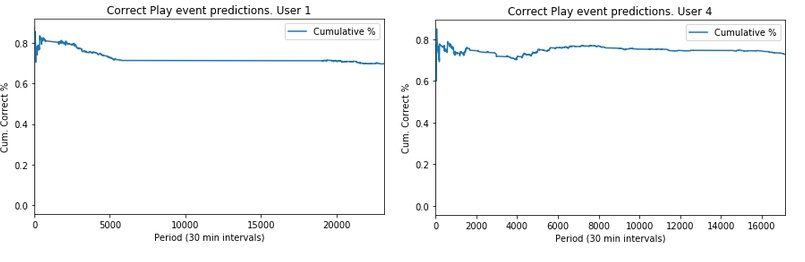
\includegraphics[width=7cm, keepaspectratio,]{fig008a.jpg}
	\caption{}
	\label{fig:fig8a}
\end{figure} 

\begin{figure}[h!]
	\centering
	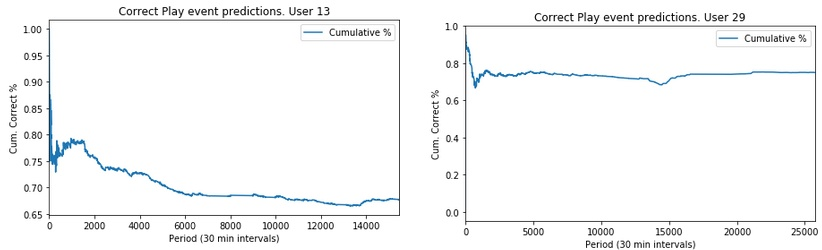
\includegraphics[width=7cm, keepaspectratio,]{fig008b.jpg}
	\caption{}
	\label{fig:fig8b}
\end{figure} 

\begin{figure}[h!]
	\centering
	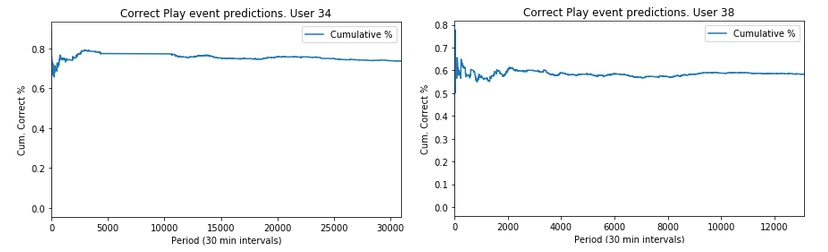
\includegraphics[width=7cm, keepaspectratio,]{fig008c.jpg}
	\caption{}
	\label{fig:fig8c}
\end{figure} 

\begin{figure}[h!]
	\centering
	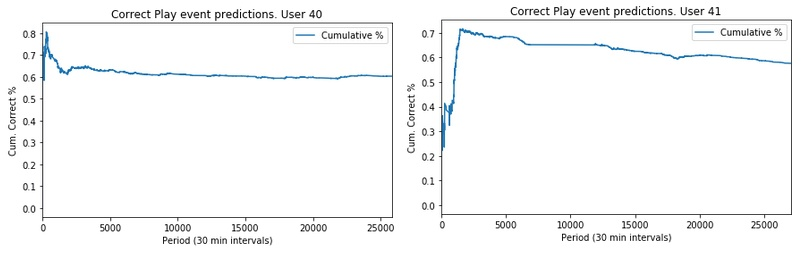
\includegraphics[width=7cm, keepaspectratio,]{fig008d.jpg}
	\caption{}
	\label{fig:fig8d}
\end{figure} 

\begin{figure}[h!]
	\centering
	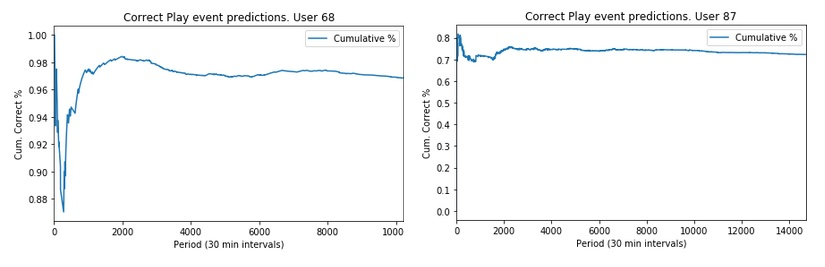
\includegraphics[width=7cm, keepaspectratio,]{fig008e.jpg}
	\caption{}
	\label{fig:fig8e}
\end{figure} 

\section{Beta-Binomial model}

\section{Logistic Regression}

\section{RNN-LSTM}

Of all the models, the RNN required the most effort to set up correctly. We provide details here to help others implementing a similar model.

\subsection{Input Shape}

In order to utilize the learning capabilities of an LSTM in Tensorflow, the input, x, must be of shape (rows,depth, cols) where rows are separate rows of training data, the depth is the time-steps that will be unrolled by the RNN, and cols are the number of features. It is important to note that when the data is unrolled, time step t for all batches are processed in one block, before t-1 , t-2 etc.

Constructung the 3-d shape often requires building them up in slices. It is highly advisable to pre-allocate the 3d array when doing this rather than extending the array on each iteration.

\subsection{Imbalanced data}

The experiments looked at the difference between feeding the RNN data rows with time lag features (t-1 .. t-5, and t-24) explictly provided, vs. excluding them and expecting the model to determine the optimal time lags for itself. A significant decrease in performance was found whehn they were excluded with recall for play events being extremely low. Further analysis indicated the recall decreases the more it is trained suggesting that the model was learnig to priotize the non-play events at the expense of play-events due to the imbalance in the data (non-play events make up ~90% of the datasete).

A weighted cost function was used to emphase play events as seen below, which led to some improvement.

